\documentclass[9pt]{beamer}

\usepackage{amsmath}
\usepackage{amsfonts}
\usepackage{listings}

\setbeamersize{text margin left=5mm,text margin right=5mm}
\setlength{\leftmargini}{3mm}
\setlength{\leftmarginii}{3mm}
% \let\Tiny\tiny% http://tex.stackexchange.com/q/58087/5764

\newcommand{\vect}[1]{\mathbf{#1}}
\newcommand{\pder}[2][]{\frac{\partial#1}{\partial#2}}
\newcommand\RR{\mathbb R}


\begin{document}
\section{pnlss}
\label{sec:generate-data}

% \begin{frame}<1>[label=pnlss]
%   \begin{center}
%     \visible<1>{Extension of PNLSS with output-based NLs}
%   \end{center}
%   \alert<1>{Generate data} \newline
%   \alert<2>{Consistency} \newline
%   \alert<3>{Nonparametric analysis} \newline
%   \alert<4>{Parametric modeling}
% \end{frame}

\begin{frame}{Extend PNLSS}
 \begin{columns}
    \begin{column}{0.5\textwidth}
      %$f_{nl} = \tanh(\dot y__{nl} \epsilon ) $
      Extend PNLSS with output-based nonlinearity.\\
      Data generated from discrete
      system\\

      \vspace{5mm}
      \centering $\vect y = [y,\, \dot y], \quad \dot y_{nl} = y_2$\\
      \centering $f_{nl} = \tanh(\dot y_{nl} / \varepsilon)$
      \begin{itemize}
      \item for high and low level: (stick or slip)\\
        Identified as linear system
      \item Intermediate level:\\
        Identified for some levels
      \item Maybe due to ``bad'' initial guess(BLA)\\
        Same behavior seen for unilateral spring
      \item Solution?\\
        Improve guess by FNSI[1](nonlinear subspace methods by J.P.)
      \item Drawbacks:\\
        - Specify $\varepsilon$ a priori\\
        - Does output(vel) correspond to slider vel?
      \end{itemize}
      \vspace{+1cm}
      \footnotesize{[1]: \url{https://doi.org/10.1016/j.ymssp.2013.06.034}}
    \end{column}
    \begin{column}{0.5\textwidth}  %%<--- here
      Validation: different $f_{nl}$ coeff.\\ Upper: 0.1*$f_{nl}$, lower: $f_{nl}$
      \begin{center}
        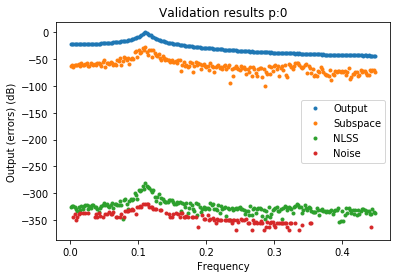
\includegraphics[width=0.9\textwidth]{fig/nlss_tahn_E1}
        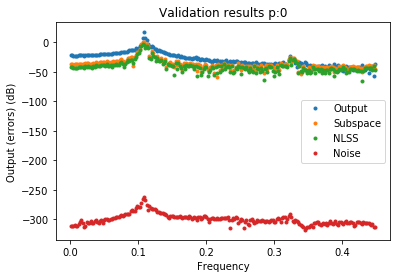
\includegraphics[width=0.9\textwidth]{fig/nlss_tahn_E10}
      \end{center}
    \end{column}
  \end{columns}
\end{frame}

\end{document}

%%% Local Variables:
%%% mode: latex
%%% coding: utf-8-unix
%%% TeX-engine: luatex
%%% magic-latex-enable-block-highlight: nil
%%% End: